\section{Analysis}

\subsection{Color Embeddings}

Intuitively we would think that making our architecture more complex and adding richer embeddings would capture the nuances of generating utterances from color embeddings. We do demonstrate this is the case in certain architectures, but adding more complexity does not necessarily lead to better performance.

\par
We find that mapping our 3-dimensional color embeddings to 54 dimensions using a Fourier transformation consistently performs the best. This is a surprising result as embedding our colors using a convolutional neural network, such as a residual network, contains much richer semantic information. There are a few explanations for why this might be.

\par
The first explanation is that while residual networks can capture rich semantic information as we encode a color with it, it is not appropriate for embedding something as simple as a color. Each layer of convolutional neural networks are supposed to find lower level features in an input image, but with a solid color there are effectively no low level features to find. So it’s likely that using the residual network as a feature extractor is actually embedding unnecessary noise into each color. We should also note that the residual networks we use in our experiments were trained on the ImageNet dataset, which requires the network to model much more complicated visual semantics than classifying a single color would.

\par
Another explanation why embedding our colors using a residual network leads to worse performance is the increase in size of our input embeddings. Our color embedding sizes go from 54-dimensional to 512-dimensional which is a more then 9x increase in dimension. This could be too large a vector for our architectures to model without fitting to noise. Putting it another way, we could be overfitting which is leading to poor generalization. This is not out of the question as our models already have several thousand learnable parameters and adding more seems to consistently make our models perform worse.

\par
A third explanation as to why our convolutional color encoder did not perform well is that we must capture more than the last layer as the color embedding. Possible options would be the element-wise sum, max, or average of the last N layers as a feature extractor. Another possibility would be to concatenate the vectors to create an \(N*512\) dimensional embedding, where \(N\) is the number of layers used in the feature extraction. This is a similar technique we use in our word embeddings, which we discuss in the following section.

\subsection{Pre-trained and Contextual Word Embeddings}

Our use of pre-trained and contextual embeddings, such as BERT, XLNet, RoBERTa and ELECTRA was motivated by a similar thought process as our color embeddings. We believed that using more powerful models that capture linguistic and semantic information would lead to better performance. Our best performing models (ELECTRA and XLNet) using pre-trained word embeddings, did not perform much better than using GloVe embeddings. All contextual word embedding models performed worse than GloVe vectors. We used contextual word embeddings output from the last layer, a combination of the last N layers, [CLS] sentence embedding, and concatenating the last layer or [CLS] and pre-trained embeddings. In all cases we observed the latter leads to improving the performance of the model.

\par
We believe the explanation for this mostly lies in our dataset used for training. The 40.8\% of our examples only contain a single word, so using contextual word embeddings would not add as much value as if the dataset would have consisted of more complex color descriptions. Using contextual embeddings requires our downstream  model to be able to effectively learn the meaning of a word embedding given its context. But given our small dataset this is likely not a feasible task leading to simply not enough complex data to capture the intricacies.

\par
Another possible explanation is that we are not producing the contextual embeddings in a way that properly captures the semantic information our model needs. Similar to the potential changes we could make to the color embedding, we could employ different methods of combining hidden layers embeddings for both the contextual word embeddings and the [CLS] sentence embedding. There are several methods we could use including the element-wise sum, max, or average of the last N layers as a feature extractor. This could include both the contextual word embeddings and the [CLS] sentence embeddings. We could even include the pre-trained word embeddings, but should note this would add a great deal of dimensionality to our models. This would increase the likelihood of building models with high variance.  We did explore this with some of our experiments resulting in poor performance. Future work might enumerate and experiment all the possible vectors and layer combinations that could potentially yield good performance.


\subsection{Sequence-to-Sequence Architecture}

We explored using two different types of RNN cells; a GRU and LSTM cell.  We found the LSTM to generally perform better than the GRU cell. The accuracy of the model using residual network color embeddings and pre-trained token embeddings improved with over 0.40 and BLEU score improved with 0.1-0.33. The accuracy of the model using Fourier color embeddings and pre-trained token embeddings improved slightly with a maximum of 0.03 but the BLEU score improved significantly with a maximum of 0.14. This is somewhat surprising as adding complexity to the other aspects of our models, such as the color embeddings and word embeddings, generally lead to worse performance.

\par
A possible explanation to this observation could be that the LSTM is inherently better at capturing long-term dependencies. This leads to a better encoding of the color representation in the last hidden state of the encoder. There are only three colors we must encode so it’s unlikely that we would get that much gain from an LSTM in the encoder. It is more likely that it is better capturing the long term dependencies of the utterances and producing utterances that are more coherent. This is reflected in the BLEU scores produced by architectures that include an LSTM cell.

\subsection{Hyperparameter Tuning}
We experimented mainly with setting different hidden dimensions for the RNN cells. In most experiments with the increase of the hidden dimension we observed an improvement of the accuracy and significant improvement of the BLEU score, with hidden dimension set to 250 performing the best. As we limited our experiments to only four dimensions settings (50, 100, 150, 250) tested with a subset of the train data (8,000 records) and the best performing models it might be that a different hidden dimension size might lead to even better performance.

\par
It is possible that with the increase of the hidden dimension size the models are able to capture additional information via the significantly increased number of trained parameters. This could potentially lead to overfitting or a better performance of the model. Data shows that the model had a slightly better performance with the dev dataset and significantly better performance with the test dataset. Consequently, we believe that the model is not overfitted but rather has captured additional information allowing it to perform better and produce significantly better English.

\subsection{Learning Efficiency}
We trained and evaluated the performance of our baseline model with GloVe, with ELECTRA and XLNet pre-trained embeddings with both GRU and LSTM cells and Fourier transformed or ResNet color representations and a hidden dimension size of 250. We also observed the efficiency of learning for those models. A set of incremental performance plots is provided on Figure \ref{figure:learning}. One can observe that all models are learning with a comparable efficiency, with the model using XLNet embeddings and Fourier transformed color representations having a higher learning efficiency.

\begin{figure*}[ht]
\centering
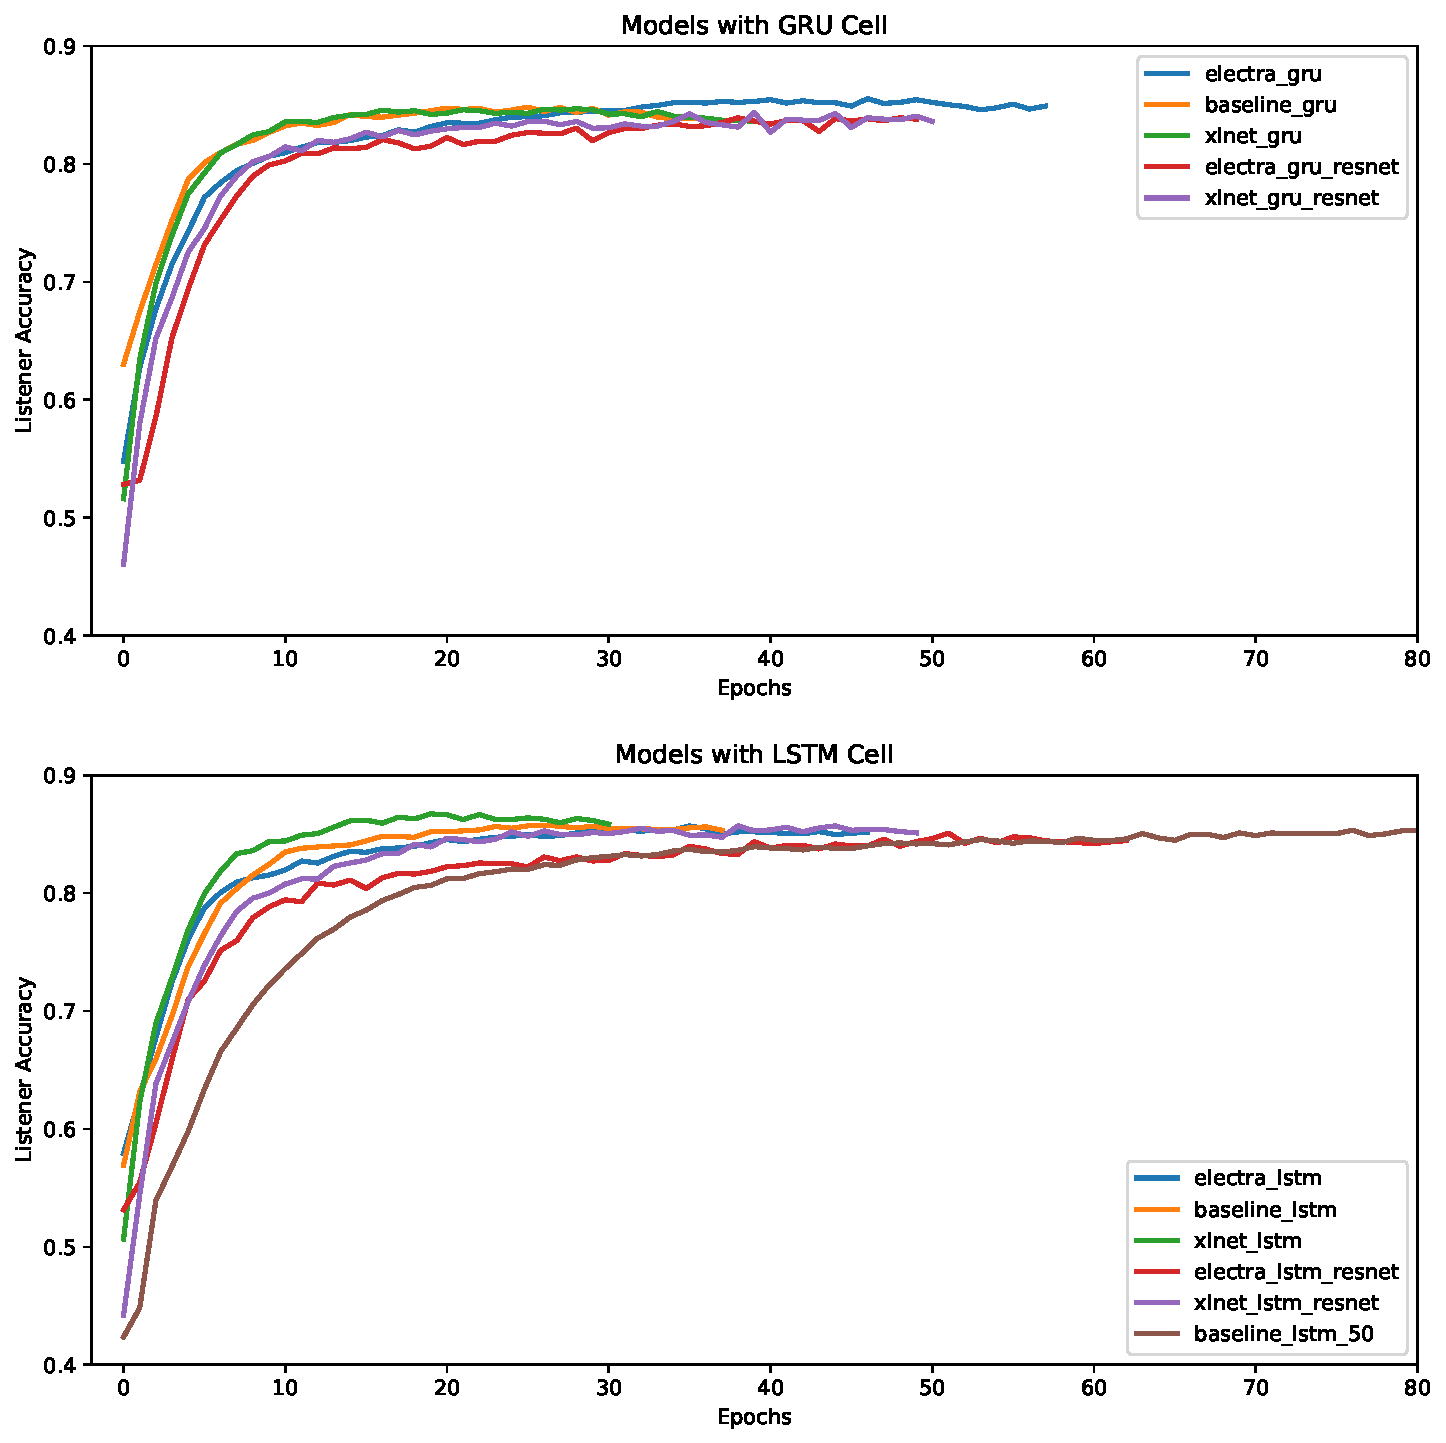
\includegraphics[width=\textwidth]{assets/learning.pdf}
\caption[Learning]{Learning efficiency of different models. XLNet embeddings have the highest learning efficiency.}
\label{figure:learning}
\end{figure*}
